\documentclass{article}

\usepackage{geometry}
\geometry{a4paper, margin=1in}

\usepackage{titlesec}
\titleformat{\section}{\large\bfseries}{\thesection.}{1em}{}
\titleformat{\subsection}{\bfseries}{\thesubsection.}{1em}{}

\usepackage{fancyhdr}
\usepackage{graphicx}
\usepackage{booktabs}
\usepackage[hidelinks]{hyperref}
\usepackage{xcolor}

\usepackage{tikz}
\usetikzlibrary{shapes,arrows,positioning}

\pagestyle{fancy}
\fancyhf{}
\rhead{\textbf{}}
\lhead{\today}
\rfoot{Page \thepage}

\begin{document}

\title{Predictive Analytics Model for the Polish Apparel Market: Integrating Domain Understanding into Strategic Business Planning}
\date{\today}
\maketitle

\newpage
\tableofcontents
\newpage

\section{Introduction}
This proposal delineates the development of a machine learning model aimed at forecasting sales trends within the Polish apparel market. Leveraging historical sales data coupled with market intelligence, the model is designed to facilitate informed decision-making in inventory management and strategic planning for a Polish trading company.

\subsection{Interview} 
The interview with the client yielded comprehensive insights into the company's business model, scale, and target demographic. Additionally, sales data was identified as a pivotal resource for our analytical model. A significant portion of the discussion centered on external factors likely to influence the company's sales, along with potential sources for data on these external elements. The conversation also clarified the project's scope, objectives, and anticipated outcomes. Furthermore, the interview provided guidance on the desired design and functionality of the application intended to deploy the trained model.

\subsection{Scope and Objectives}
The primary objective of this project is to construct a predictive analytics model that accurately forecasts sales trends in the Polish apparel market. This model is intended to support efficient inventory management and enhance strategic decision-making processes.


\subsection{Expanded Market Understanding}
Poland's market, demands a comprehensive understanding of various product categories, effective sales strategies, and an awareness of external factors influencing sales. This document integrates an in-depth understanding of these nuances, enhancing the model's contextual relevance.

\section{Business Model}
The company operates based on a direct sourcing and distribution model, which can be described in the following steps:

\begin{enumerate}
    \item \textbf{Product Design and Sourcing:} 
    The company either sources pre-designed products or creates custom designs tailored to specific needs. For custom designs, the company conceptualizes the design and then collaborates with manufacturing entities in China to bring these designs to life.

    \item \textbf{Production:} 
    With the designs in hand, the products are then manufactured in specialized factories located in China. These factories are equipped to produce protective gear that meets both the design specifications and any required safety standards.

    \item \textbf{Distribution and Sales:} 
    Once the products are manufactured and ready for the market, the company takes on the role of distributor. They sell these products to:
    \begin{itemize}
        \item DIY shops, like Leroy Merlin.
        \item Wholesalers who specialize in the distribution of protective gear.
    \end{itemize}

    \item \textbf{End Consumers:} 
    The DIY shops and wholesalers, in turn, sell these products to the end consumers. The primary target for these products are companies that require protective gear for their industrial operations. However, there is also a retail segment where individual consumers can purchase these products for personal use.
\end{enumerate}

Here is visualization of above described business model:

\begin{center}
    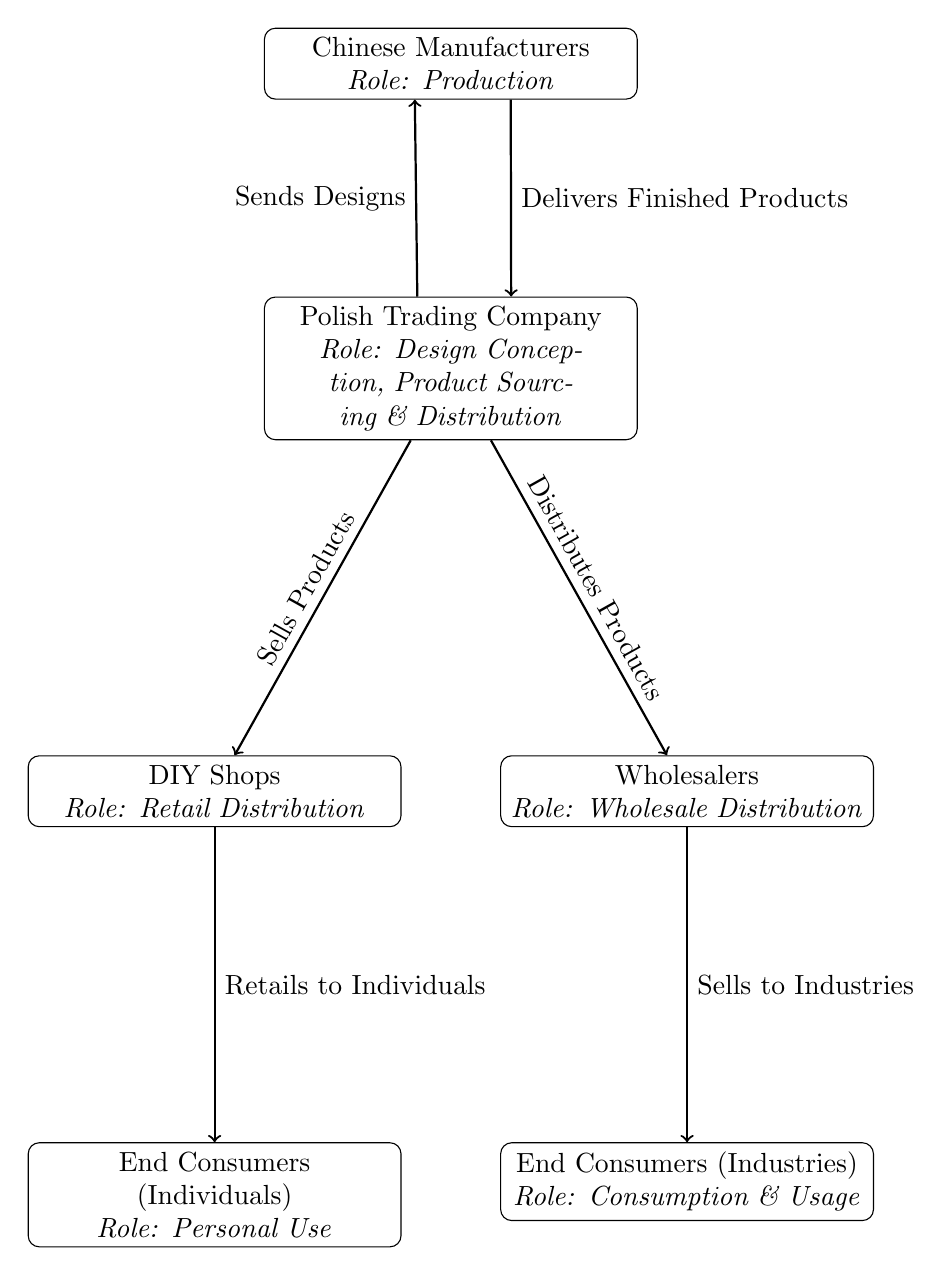
\begin{tikzpicture}[node distance=2.5cm, auto]
        % Nodes
        \node[draw, rectangle, rounded corners, text width=4.5cm, align=center] (company) {Polish Trading Company \\ \textit{Role: Design Conception, Product Sourcing \& Distribution}};
        \node[draw, rectangle, rounded corners, text width=4.5cm, align=center, above=of company] (manufacturers) {Chinese Manufacturers \\ \textit{Role: Production}};
        \node[draw, rectangle, rounded corners, text width=4.5cm, align=center, below=of company, yshift=-1.5cm, xshift=-3cm] (shops) {DIY Shops \\ \textit{Role: Retail Distribution}};
        \node[draw, rectangle, rounded corners, text width=4.5cm, align=center, below=of company, yshift=-1.5cm, xshift=3cm] (wholesalers) {Wholesalers \\ \textit{Role: Wholesale Distribution}};
        \node[draw, rectangle, rounded corners, text width=4.5cm, align=center, below=of shops, yshift=-1.5cm] (individuals) {End Consumers (Individuals) \\ \textit{Role: Personal Use}};
        \node[draw, rectangle, rounded corners, text width=4.5cm, align=center, below=of wholesalers, yshift=-1.5cm] (consumers) {End Consumers (Industries) \\ \textit{Role: Consumption \& Usage}};
    
        % Arrows
        \draw[->, thick] (company.115) -- (manufacturers.945) node[midway, left, align=center] {Sends Designs};
        \draw[->, thick] (manufacturers.689) -- (company.50) node[midway, right, align=center] {Delivers Finished Products};
        \draw[->, thick] (company) -- (shops) node[midway, above, sloped, align=center] {Sells Products};
        \draw[->, thick] (company) -- (wholesalers) node[midway, above, sloped, align=center] {Distributes Products};
        \draw[->, thick] (shops) -- (individuals) node[midway, right, align=center] {Retails to Individuals};
        \draw[->, thick] (wholesalers) -- (consumers) node[midway, right, align=center] {Sells to Industries};
    \end{tikzpicture}
    \end{center}

    \section{Key Considerations}
    \begin{itemize}
        \item \textbf{Sales Planning:} Preparation is crucial. When approaching large retail chains, businesses must anticipate their needs. This might mean bolstering their workforce in advance of significant sales events, ensuring that customer demands are met efficiently.
        \item \textbf{Market Trends:} Poland boasts a unique blend of local and international fashion preferences. Recognizing and catering to this balance can set a business apart, allowing them to connect more effectively with their target audience.
    \end{itemize}

    \section{Categorizing Apparel}
    Understanding the different categories of apparel can help businesses strategize effectively.
    \subsection{By Demand}
    \begin{itemize}
        \item \textbf{Seasonal Apparel:} Products like winter jackets and summer sandals are influenced by the changing seasons. Anticipating these shifts can lead to optimized sales.
        \item \textbf{Evergreen Apparel:} Certain staples, such as t-shirts and jeans, are consistently in demand, making them essential inventory items.
    \end{itemize}
    \subsection{By Function}
    \begin{itemize}
        \item \textbf{Upper Body Wear:} This category, including jackets and shirts, is vast and caters to both daily wear and specific occasions.
        \item \textbf{Headgear:} From fashionable hats to protective helmets, this category serves both function and style.
        \item \textbf{Leg Wear and Protection:} Beyond daily wear like trousers, this category also includes specialty items like protective gear.
    \end{itemize}

    \section{Effective Sales Approaches}
    \begin{itemize}
        \item \textbf{Bundling Products:} Offering products as sets, such as a jacket with matching gloves, can enhance sales appeal. Such bundles can offer customers better value and enhance their shopping experience.
        \item \textbf{Identifying Target Audiences:} A clear understanding of the target market, whether it's the general public or niche groups, can lead to more tailored and effective sales strategies.
    \end{itemize}

\section{Influences on Sales}
Numerous external factors can sway consumer purchasing decisions.
\begin{itemize}
    \item \textbf{Economic Climate:} The broader economic health can influence consumer spending habits, with downturns leading to more conservative buying behavior.
    \item \textbf{Fashion Shifts:} The ever-evolving world of fashion can drastically impact the popularity of certain apparel items.
    \item \textbf{E-commerce Trends:} As the digital age progresses, online shopping continues to reshape traditional buying patterns.
    \item \textbf{Regulatory Environment:} Changes in government regulations, trade policies, or import/export tariffs can affect both sales and manufacturing practices.
    \item \textbf{Sustainability Concerns:} With increasing global emphasis on eco-friendly practices, sustainable and ethically-produced apparel is gaining traction.
\end{itemize}

\section{Understanding Sales Data}
\begin{itemize}
    \item \textbf{Data Source:} Analyzing company-specific sales data for market performance insights.
    \item \textbf{Leveraging Data:} Utilizing data analysis to predict consumer behavior and market trends, refining business strategies.
\end{itemize}



\section{Data Sourcing}

\subsection{Data Sources}
This project will utilize a dual-source approach for data acquisition, encompassing both internal company records and external data provided by Polish government sources. This blend of data sources will offer a comprehensive view of the market, aiding in the development of a robust predictive model.

\begin{itemize}
    \item \textbf{Company Sales Data:}
    \begin{itemize}
        \item Historical sales records from the company will form the primary dataset. This includes transaction data, product categories, sales volumes, and revenue figures over multiple time periods.
    \end{itemize}
    
    \item \textbf{Polish Government Sources:}
    \begin{itemize}
        \item \textit{Inflation Data:} Inflation rates provided by the National Bank of Poland or the Central Statistical Office will be used to understand the economic climate and its impact on consumer purchasing power.
        \item \textit{Temperature Data:} Climatic data, specifically temperature records from the Institute of Meteorology and Water Management, will be analyzed to assess their correlation with seasonal sales trends in the apparel market.
        \item \textit{Unemployment Rates:} Unemployment statistics from the Central Statistical Office will be incorporated to evaluate the influence of employment levels on consumer spending patterns in the apparel sector.
    \end{itemize}
\end{itemize}

This comprehensive dataset, encompassing both internal sales metrics and external economic indicators, will provide a robust foundation for the predictive model. It will allow for the analysis of diverse factors influencing the apparel market, enabling more accurate and nuanced predictions.


\subsection{Data Collection Methods}
The data collection for this project will be meticulously executed, utilizing a variety of methods to gather comprehensive data from both internal company records and external government sources. The methodology ensures accurate and up-to-date information, crucial for the effectiveness of the predictive model.

\begin{itemize}
    \item \textbf{Internal Company Data Extraction:}
    \begin{itemize}
        \item Data from internal company records, particularly historical sales data, will be extracted using automated data retrieval systems. This will include sales volumes, revenue figures, and product categories.
    \end{itemize}
    
    \item \textbf{External Data Retrieval:}
    \begin{itemize}
        \item \textit{Inflation and Unemployment Rates:} Data on inflation and unemployment rates will be sourced from the official websites of the National Bank of Poland and the Central Statistical Office, respectively, using web scraping techniques.
        \item \textit{Temperature Data:} Climatic data, such as temperature records, will be collected from the Institute of Meteorology and Water Management's official portal.
        \item All external data will be verified for accuracy and relevance, and cross-checked with alternative sources where available.
    \end{itemize}
\end{itemize}

This diverse approach to data collection will ensure a rich dataset, combining precise internal sales metrics with macroeconomic indicators and environmental factors, to build a comprehensive predictive model.



\subsection{Objectives}

The objectives for data sourcing in this project include identifying and collecting high-quality, relevant data that will be instrumental in training the predictive model. The focus is on acquiring data that provides comprehensive insights into the Polish apparel market.

\subsection{Data Requirements}

Data requirements encompass the need for historical sales data, market trends, consumer behavior analytics, and any other relevant data that can enhance the model's accuracy and relevance.


\subsection{Data Legality and Ethics}

Data sourcing will adhere to all legal and ethical standards, ensuring respect for privacy laws and intellectual property rights.

\subsection{Data Diversity}

A diverse range of data will be sought to ensure the model's robustness and ability to generalize across various market segments and consumer demographics.

\subsection{Version Control}

Effective version control mechanisms will be employed to track changes in data sourcing and preparation, enhancing the reproducibility and reliability of the model.

\section{Analytic Approach}
The analytic framework of this project involves deploying advanced machine learning algorithms to scrutinize the collected data. The objective is to engineer a model capable of precisely forecasting sales trends, thereby contributing valuable insights for strategic business decisions.


\subsection{Machine Learning Techniques}

Various machine learning techniques, such as regression analysis, classification algorithms, and time-series forecasting, will be evaluated to select the most appropriate method for the predictive model.

\subsection{Model Validation and Testing}

The model will undergo rigorous validation and testing processes to ensure its accuracy and reliability. This will include cross-validation techniques and performance metric assessments.

\subsection{Deployment Strategy}

A detailed deployment strategy will be developed for  This will include plans for model integration, monitoring, and continuous improvement.


\subsection{Model Evaluation Metrics}
Apply metrics such as MAE, R-squared, and precision-recall for evaluating different aspects of the model's performance.


\section{Conclusion}
This proposal articulates a comprehensive strategy for the creation of a predictive analytics model, tailored to the nuances of the Polish apparel market. Integrating a profound understanding of market dynamics with sophisticated data sourcing and analytic methodologies, this project aims to revolutionize the approach to strategic business planning and decision-making.


\end{document}